\documentclass[class=ctexart,crop=false]{standalone}

\usepackage{amsmath,amssymb,enumitem,empheq,tkz-euclide,
diagbox,wrapfig,pgfplots,geometry}
%\geometry{a4paper,scale=0.9}
\pgfplotsset{compat=newest}
%\usepgfplotslibrary{external}
%\tikzexternalize
\renewcommand\parallel{\mathrel{/\mskip-2.5mu/}}

\newcommand\px{\mathrel{/\mkern-5mu/}}  %平行
\newcommand\pxeq{\mathrel{\vcenter{     %平行且等于
\ialign{\hfil##\hfil\crcr
$\scriptstyle\px\!$\crcr
\noalign{\nointerlineskip\vskip1pt}$=$\crcr}}}}

%\setCJKmainfont{SimSun}       %设置西文字体为times new roman
%\setCJKsansfont{SimSun}             %设置中文字体为宋体
%\setCJKmonofont{STKaiti}
%\setsansfont{TeX Gyre Termes}            %设置typewriter family中文字体为楷体
%\setmonofont{TeX Gyre Termes}

\usetikzlibrary{calc,intersections,through,backgrounds,patterns}
\newcounter{para}
\newcommand\mypara{\par\refstepcounter{para}\thepara.\space}%设置typewriter family西文字体为times new roman
\newcommand*\circled[1]{\tikz[baseline=(char.base)]{
            \node[shape=circle,draw,inner sep=1pt] (char) {#1};}}

\newcommand{\rnum}[1]{\romannumeral #1}
\newcommand{\RNum}[1]{\uppercase\expandafter{\romannumeral #1\relax}}
\begin{document}
四边形 $ABCD$ 中, $\angle ABC=50^\circ, 
\angle DBC=30^\circ,\angle BAC=60^\circ,
\angle DAC=20^\circ.$ 求 $\angle ACD$\hfill\hphantom\quad
\begin{wrapfigure}{r}{0.25\textwidth}
    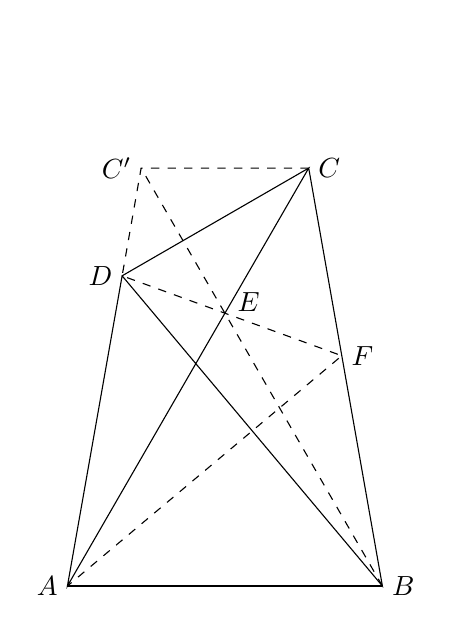
\begin{tikzpicture}
        \coordinate[label={180:{$A$}}] (A) at (-2,0) {};
        \coordinate[label={0:{$B$}}] (B) at (2,0) {};
        \path[name path=elAC] (A)--($(A)!1.7!60:(B)$);
        \path[name path=elBC] (B)--($(B)!-1.5!100:(A)$);
        \path[name path=elAD] (A)--($(A)!1.8!80:(B)$);
        \path[name path=elBD] (B)--($(B)!-1.7!130:(A)$);
        \path[name intersections={of=elAC and elBC,by={[label=right:$C$]C}}];
        \path[name intersections={of=elAD and elBD,by={[label=left:$D$]D}}];
        \draw[] (D)--(A)--(C)--(D)--(B)--(C);
        \draw[] (A)--(B);
        \path[name path=elBC'] (B)--($(B)!-1.8!120:(A)$);
        \path[name intersections={of=elAD and elBC',by={[label=left:$C'$]C'}}];
        \path[name intersections={of=elAC and elBC',by={[label={[shift={(.3,-.1)}]$E$}]E}}];
        \path[name path=elDE] (D)--($(D)!2.4!(E)$);
        \path[name intersections={of=elDE and elBC,by={[label=right:$F$]F}}];
        \draw[dashed] (C)--(C')--(D)--(F)--(A);
        \draw[dashed] (B)--(C');
    \end{tikzpicture}
\end{wrapfigure}
解:\\
过 $C$ 作 $CC' \parallel AB $ 并交 $AD$ 的延长线于 $C'$连接 $C'B$ 交 $AC$ 于 $E'$,连接 $DE$ 
并延长, 交 $BC$ 于 $F$,连接 $AF.$\\
$\angle BAC'=60^\circ+20^\circ=80^\circ$\\
$\angle ABC=50^\circ+30^\circ=80^\circ=\angle BAC'$\\
又 $CC'\parallel AB$故 $ABCC'$为等腰梯形\\
据对称性,$\angle ABC'=\angle BAC=60^\circ$\\
故 $\triangle ECC',\triangle ABE$ 为正三角形,则 $AE=AB$\\
$\triangle ABD$ 中:\\ 
$\angle ADB=180^\circ-50^\circ-80^\circ=50^\circ=\angle ABD$\\
故 $AD=AB=AE$\\
在 $\triangle ADE$ 中, $\angle ADE=\angle AED=80^\circ$\\
则 $\angle BDF=30^\circ=\angle DBF,\angle CDC'=100^\circ$\\
故 $\triangle BDF $为等腰三角形,$DF=BF$\\
又 $AF=AF,AD=AE$则 $\triangle AFD \cong \triangle AFB$\\
故 $\angle BAF=\frac{1}{2}\angle DAB=40^\circ$\\
$\triangle ABF$中 $\angle BFA=180^\circ-40^\circ-80^\circ=60^\circ$\\
$\triangle BEF$中 $\angle BEF=180^\circ-\angle BFE-\angle EBF=40^\circ$\\
而 $\angle AC'B=180^\circ-\angle C'AB-\angle C'BA=40^\circ=\angle BEF=\angle C'EF$\\
故 $\triangle C'DE$ 为等腰三角形, $C'D=DE$\\
又 $\triangle CC'E$为正三角形, $CC'=CE$\\
又 $CD=CD$,故 $\triangle CC'D \cong \triangle CED$\\
而 $\angle C'CE=180^\circ-\angle CBA=100^\circ$\\
$\angle ACB=\angle AC'B=40^\circ$\\
故 $\angle ACD=\frac{1}{2}\angle C'CA=\frac{1}{2}(100^\circ-40^\circ)=30^\circ$
\end{document}